\section{System's Perspective}
\subsection{Overview of Minitwit}
\begin{figure}[H]
    \centering
    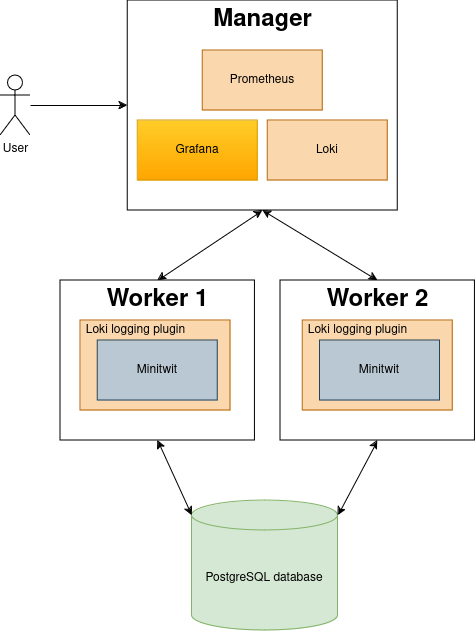
\includegraphics[scale=.7]{diagrams/overall_system.png}
    \caption{Diagram showing the docker swarm structure of Minitwit}
    \label{fig:overall_system}
\end{figure}
Figure \ref{fig:overall_system} shows an overview of our final setup. Our setup is using docker swarm to distribute the workload between multiple instances of minitwit. In our current system we have 3 nodes, 1 manager and 2 workers. The manager contains running instances of \textit{Prometheus} for collecting metrics, \textit{Loki} for collecting logs and \textit{Grafana} to visualize our metrics and logs.
\\
\\
Each of our worker nodes run their own instance of the Minitwit application. When the Minitwit application wants to log something it just prints it to the standard output. We then have a Loki logging plugin attached to the container, which will send whatever is printed to standard output to the running Loki instance on the Manager. The Minitwit applications both use the same PostgreSQL database, which ensures consistent data. The only internal state that the Minitwit application has is its metrics, which the Prometheus instance on the manager will then collect, and that we can then aggregate and show in Grafana. 

% \subsection{Client Architecture}
% The first refactor of Minitwit used Go's HTML templates to serve as a frontend interface for users \cite{gotemplates}. The implementation followed closed to the Python templates from the pre-refactored minitwit application.
% \\
% \\
% Soon after we noticed a few problems with the templating for the client interface. First of all, templates were served through our Go backend. The logic between frontend and backend was tightly coupled, leading to unexpected software behaviours. Moreover, we had difficulties in scaling our system with new features. Writing and changing HTML templates was hard to understand and debug.
% \\
% \\
% All of the above-mentioned problems led to a group discussion to find a better alternative to solve this problem. Even though the system was fully implemented for client interface features, we still wanted to show that we can create a more robust client architecture which separates the logic from the backend.
% \\
% \\
% We decided to switch the frontend to use React \cite{react}. A few of us had previously worked with React, therefore, it was an easy choice to save time and show that we can scale the system for future. Most implementation details are left for the reader on the GitHub repository. The important change from HTML templates to React is shown in figure \ref{fig:react-dev}.

% \begin{figure}[H]
%     \centering
%     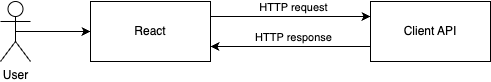
\includegraphics[scale=.6]{diagrams/react-dev.png}
%     \caption{Diagram to depict user interactions with the backend through React.}
%     \label{fig:react-dev}
% \end{figure}

% Instead of Go serving HTML templates, Go serves a React bundle with which the user interacts. React can then encode more complex interactions between the frontend and the backend. Furthermore, the client is fully decoupled separating the logic from the backend. Lastly, React is written in JavaScript which eases development with a large community support.
% \\
% \\
% Finally, deployment process to production had to be changed as well. This meant that the docker build had to create not only the Go binary of the backend but also build React into a suitable format any browser would run. Figure \ref{fig:react-prod} displays what docker image is pushed to the VPS on DigitalOcean.

% \begin{figure}[H]
%     \centering
%     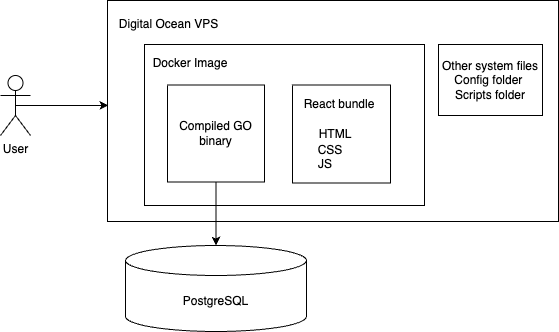
\includegraphics[scale=.7]{diagrams/react-prod.drawio.png}
%     \caption{User interactions when accessing deployed Minitwit.}
%     \label{fig:react-prod}
% \end{figure}

% The user entering the VPS hits a running Go server from the docker image. If the user asks for a page, the Go API will serve the built React bundle which will usually have a root HTML page, a few JavaScript and CSS files. User's browser will then rebuild the React interface locally from the mentioned files. The user will continue to interact with the website through React as a helper tool to communicate with the Go API which will handle the rest of the backend logic.

% \subsubsection{E2E Testing}
% One of the benefits of using React is its rich tool palette. One of the tools built by Microsoft is a modern end-to-end testing library - Playwright \cite{playwright}. Playwright integrates seemingly with React, offering great developer experience. We have implemented this library for our client testing to test different end-to-end actions: user register/login, following and tweeting. The documentation is extensive with parallel tests running in different browsers, screenshots for failed tests, CI integrations, interactive app and many more.
% \\
% \\
% Figure \ref{fig:playwright-terminal} displays running Playwright test, where the instructions were defined by us under [name].spec.ts files. The same tests are running on each pull request as part of the CI actions to make sure the frontend behaviours work as expected.

% \begin{figure}[H]
%     \centering
%     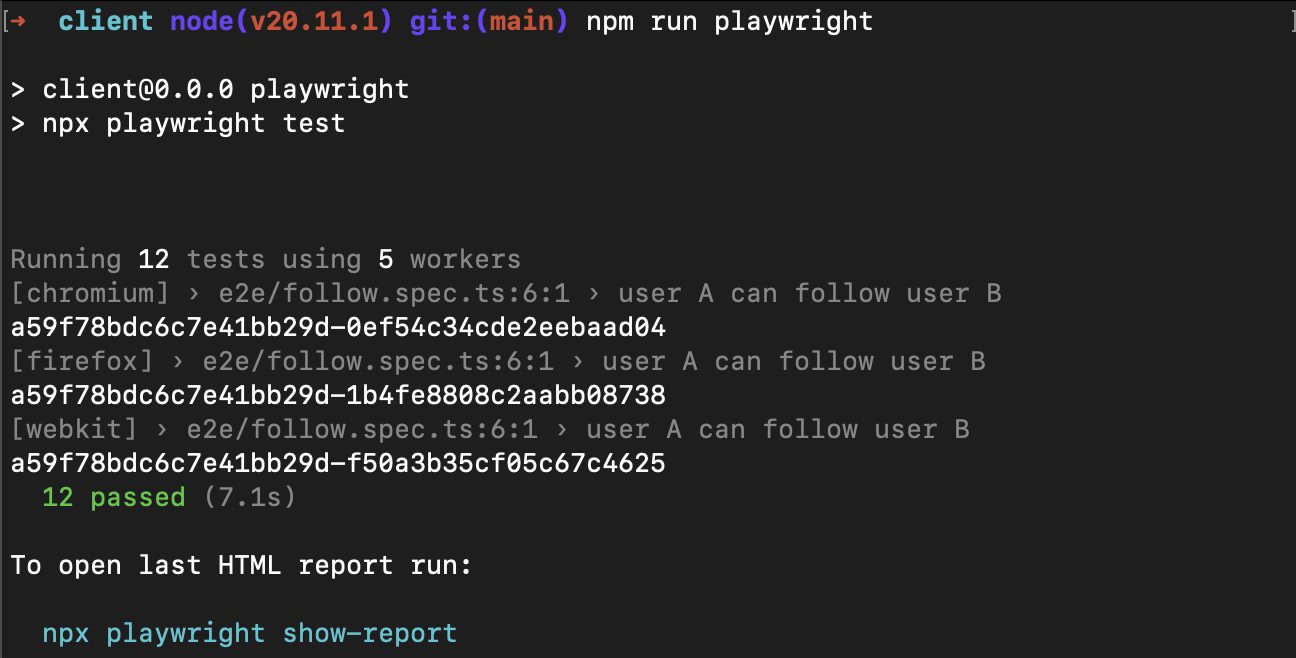
\includegraphics[scale=.3]{img/playwright-terminal.png}
%     \caption{Playwright running E2E tests.}
%     \label{fig:playwright-terminal}
% \end{figure}

% For more in-depth analysis of the completed tests, Playwright generates a report, shown in figure \ref{fig:playwright-report}. The same report is attached as an artifact under the CI actions on GitHub, allowing developers to analyse any failed or successful E2E tests.

% \begin{figure}[H]
%     \centering
%     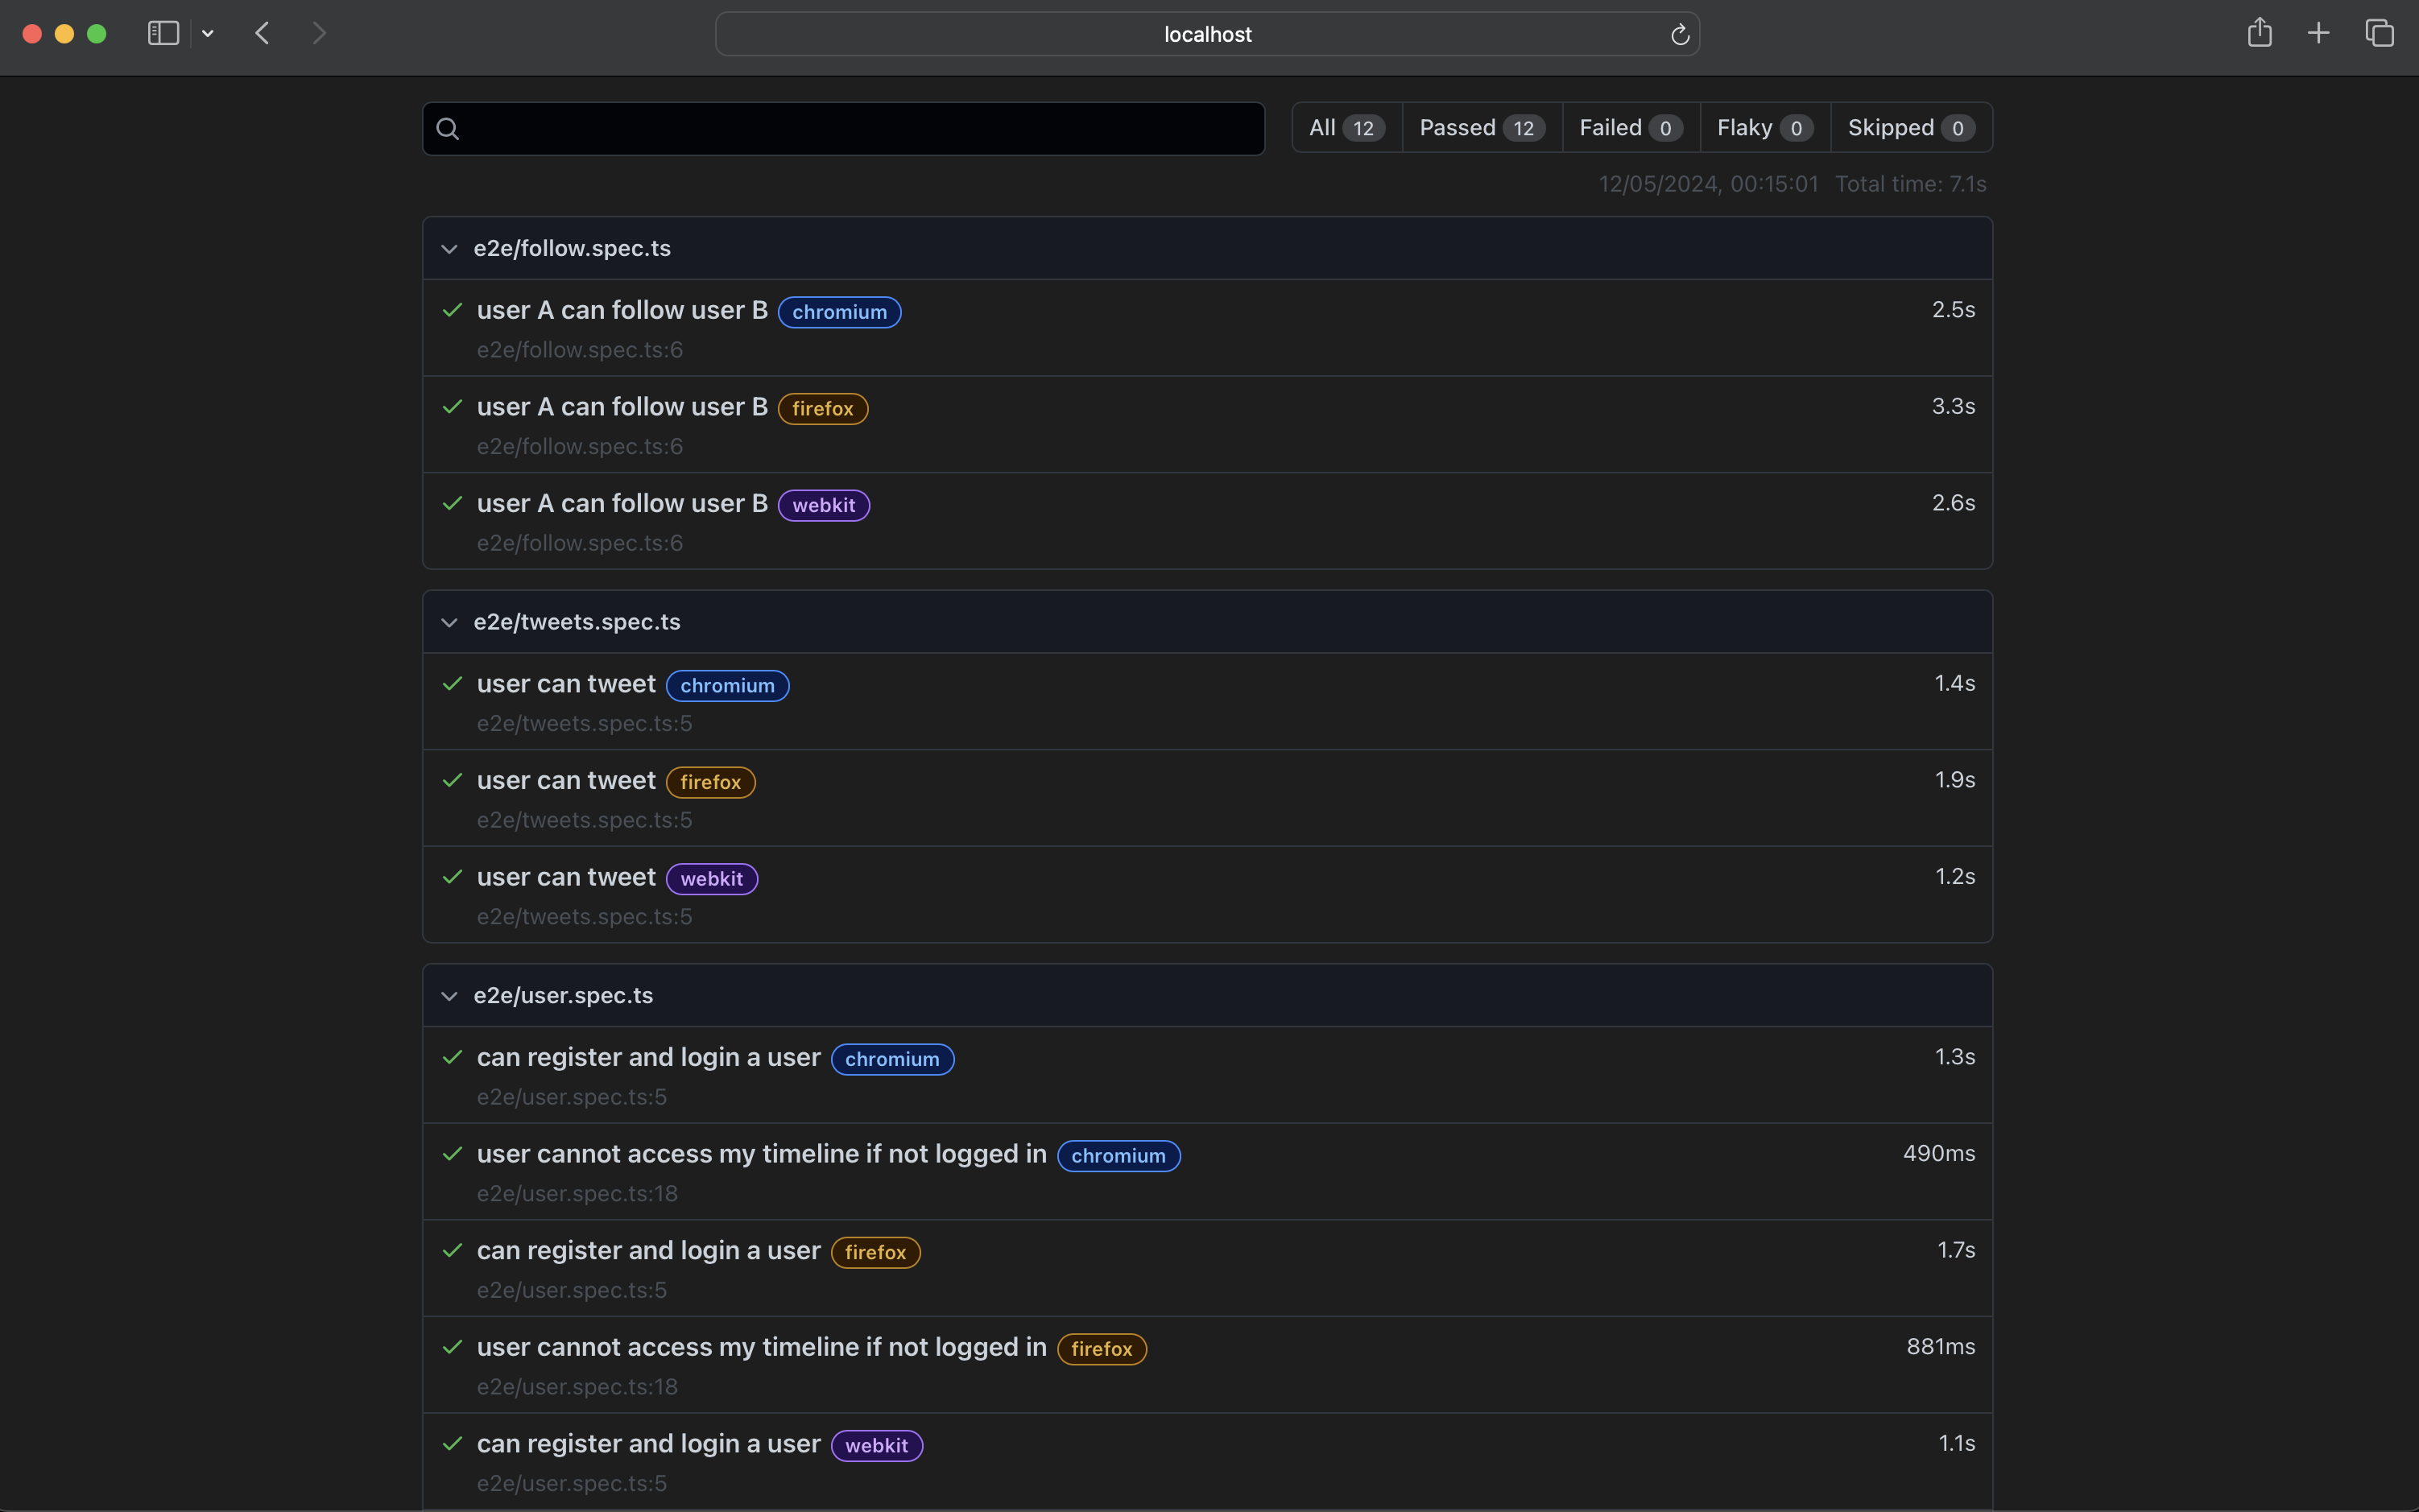
\includegraphics[scale=.15]{img/playwright-report.png}
%     \caption{Playwright's generated test report.}
%     \label{fig:playwright-report}
% \end{figure}

% The last worth mentioning feature is Playwright's integrated app shown on figure \ref{fig:playwright-app}. The app is opened by running one of the terminal cli commands. With the app, the developers can visually inspect all running tests on different defined browsers and debug any issues that arise. 

% \begin{figure}[H]
%     \centering
%     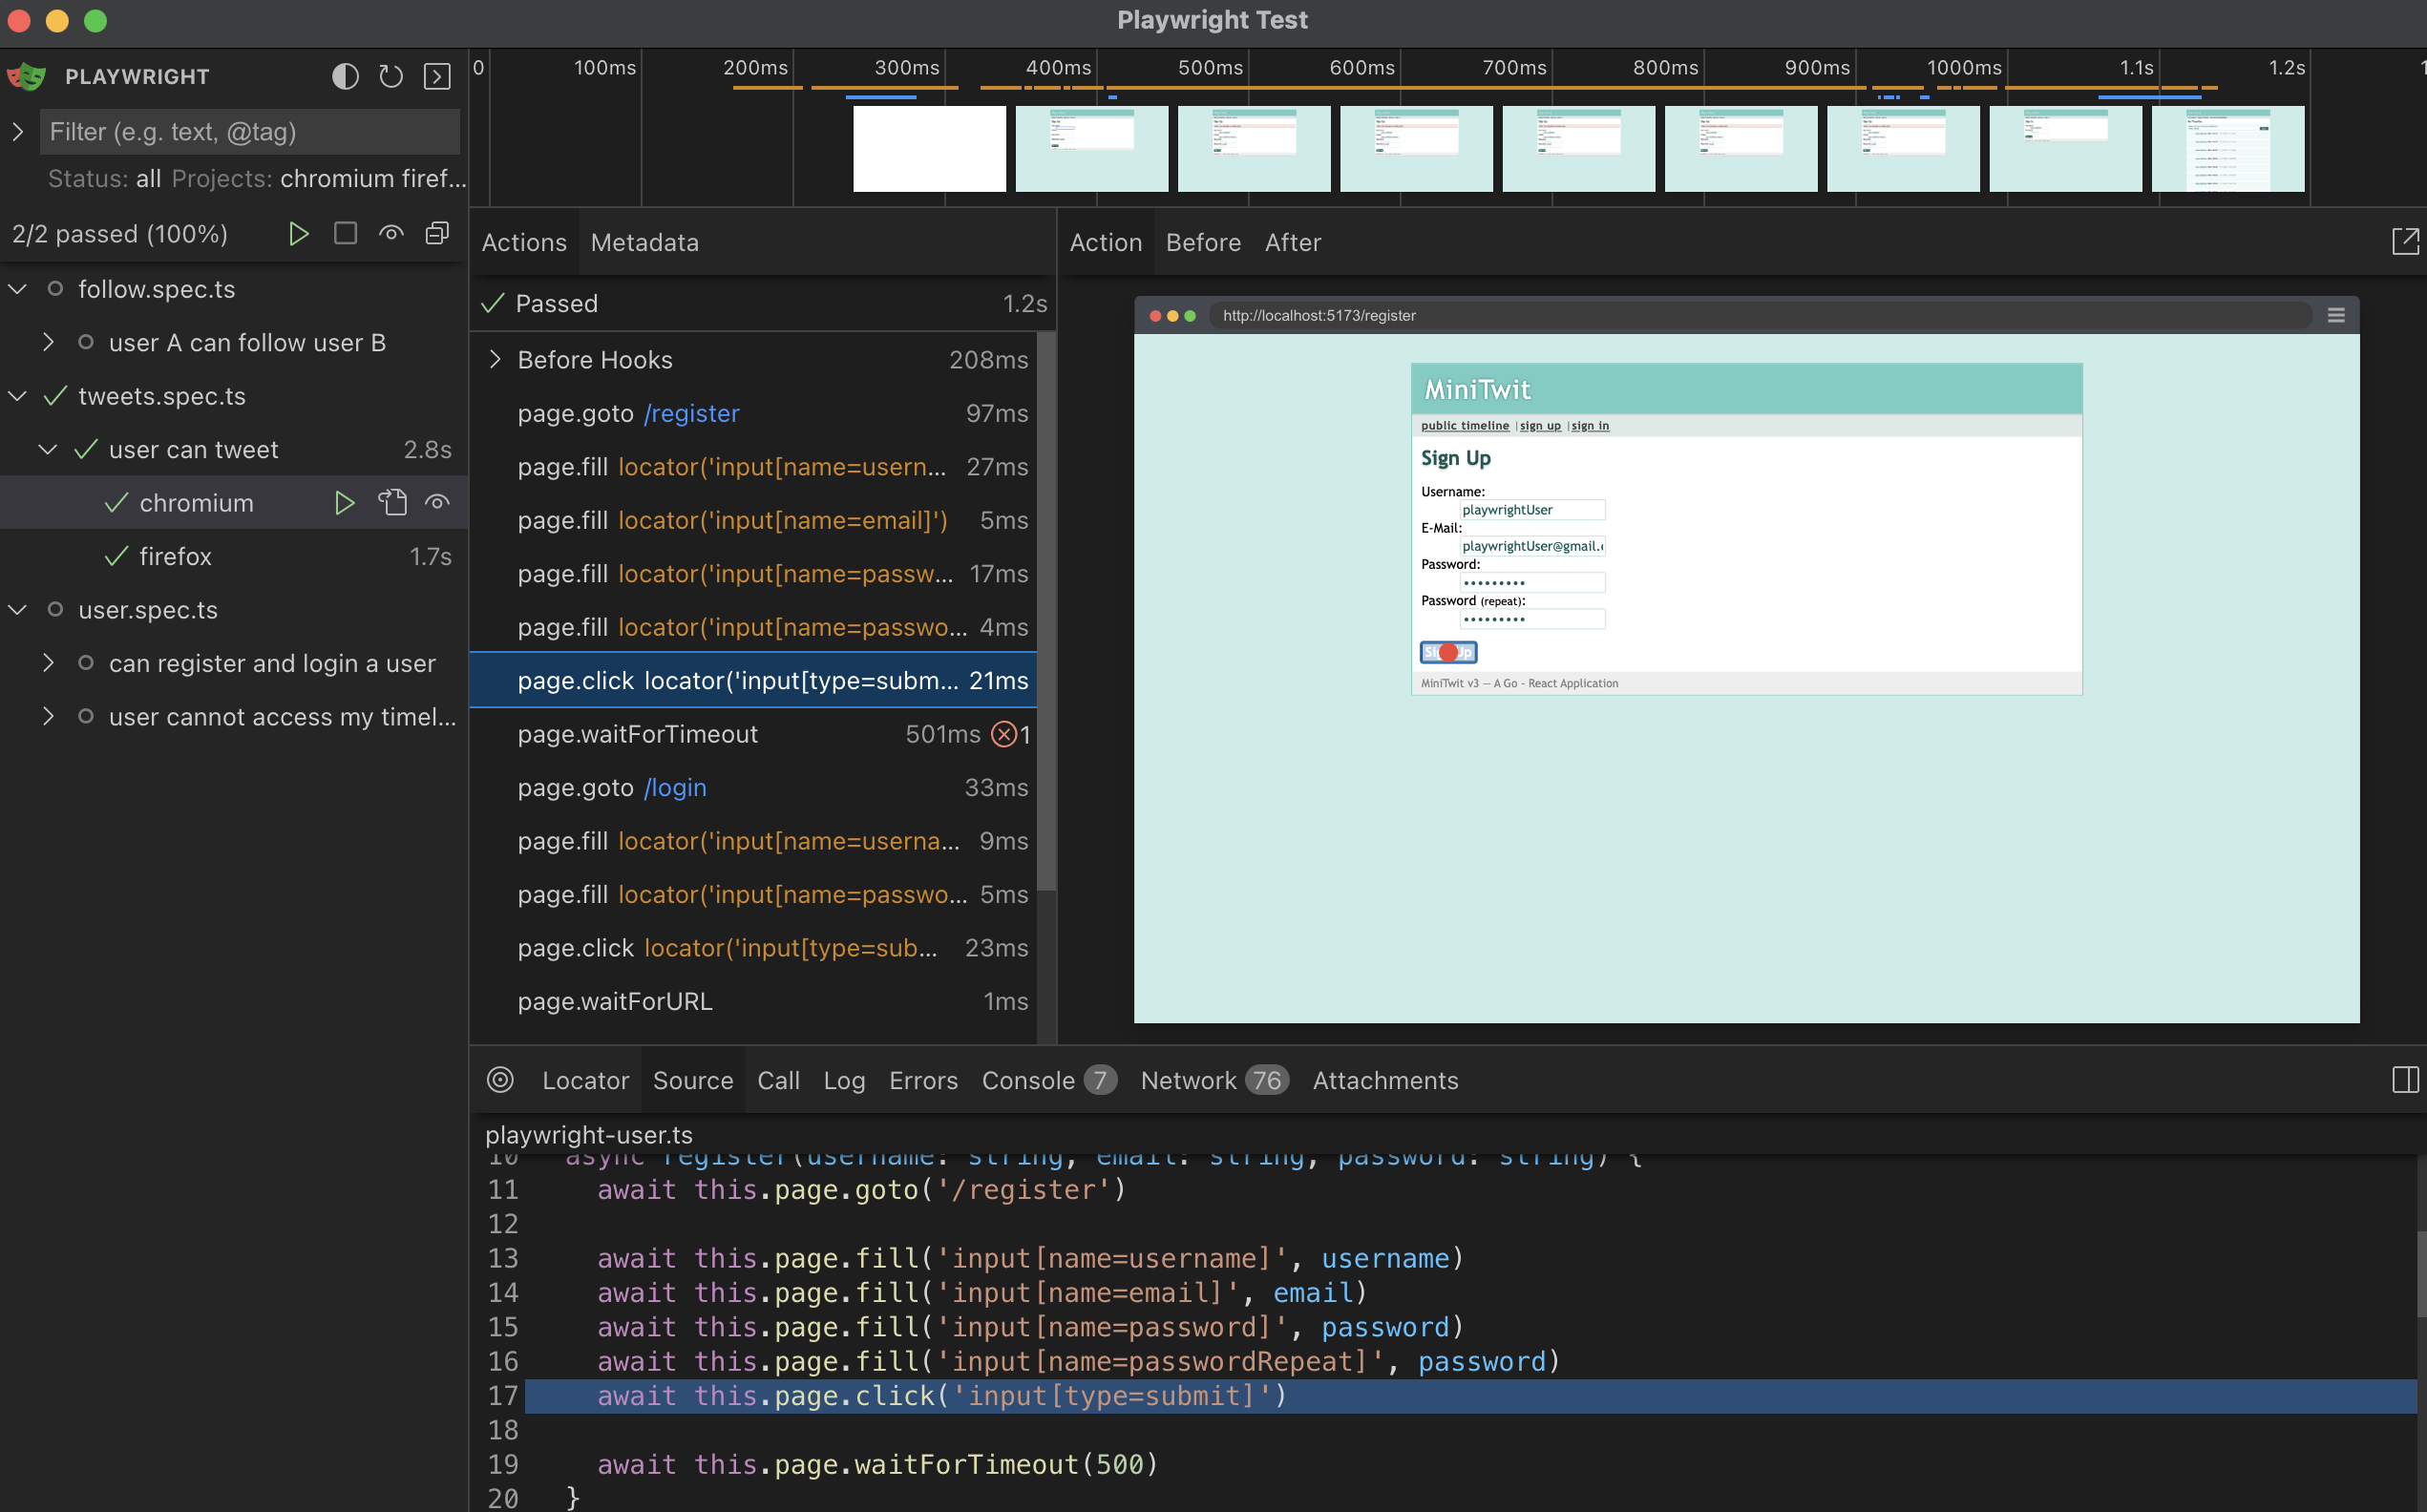
\includegraphics[scale=.18]{img/playwright-app.png}
%     \caption{Playwright's app to visualize and debug tests.}
%     \label{fig:playwright-app}
% \end{figure}

\subsection{Dependencies of Minitwit}

\subsubsection{Application Dependencies}
We decided to do our refactoring of Minitwit in the language Go. The reason for this is that it is the language that one of our group members had the most experience with for backend development, and the rest of the group wanted to learn the language. The language has a solid standard library for writing backends, as well as a great ecosystem with useful libraries. The language also has support for rendering templates that are very similar to the flask templates used in the old Python 2 Minitwit, which made the initial 1-to-1 refactor easier to do.
\\
\\
For interacting with the database, we decided to use the ORM (Object-relational Mapping) called \textit{GORM} \cite{gorm}. This made it easier to interact with the database and map data to objects that we could then use more easily. It also made it easier to modify the setup of the database, for example when creating indexes to speed up queries.
\\
\\
Our other major dependency is the library called \textit{Gorilla} \cite{gorilla}, which makes handling things like cookies and API routing much simpler and adds useful functionality. Both GORM and Gorilla were something we were familiar with, as to why we chose to use them. 
\\
\\
For monitoring we chose to use \textit{Prometheus}, \textit{Grafana} and the built in tools from Digital Ocean. We chose \textit{Prometheus} and \textit{Grafana} because we were introduced to them in class and it seemed like they were tools that were used in the real world. \textit{Prometheus} also had the added benefit of being easy to integrate into our Go backend.
\\
\\
For logging we decided to use \textit{Loki}, as \textit{Grafana} had built in support for it. Initially we used \textit{Promtail} to retrieve data from standard output and send it to \textit{Loki}, but after switching our system to use Docker Swarm we ended up using a Loki logging plugin for our containers.
\\
\\
For the frontend we started out by using the templates that are part of Go, but switched to a React frontend. We did this because it had more features and a better development experience. Multiple members of the group already had experience with React, and the rest wanted to use this course as an opportunity to learn it.

\subsubsection{Infrastructure dependencies}
As a provider for our servers we chose \textit{Digital Ocean}. It was one of the suggestions from the course and some of the group members already have had experience with it. It also helped that we were able to get free credits since we were students.
\\
\\
For running our different services we chose \textit{Docker}. It made handling dependencies much easier, and some of the services, like \textit{Grafana} and \textit{Loki}, already had readily available images for us to use with little setup. We used \textit{Docker Compose} to run all of our services with one file. Later we decided to use \textit{Docker Swarm} to do load-balancing, as it fit well with our setup at the time and was easy to set up. Using \textit{Docker Compose} and \textit{Docker Swarm} made also easy to do continuous deployment with little-to-no downtime.
\\
\\
For creating our virtual machines, referred to as \textit{Droplets}, we initially used Vagrant as we were introduced to it in class. We weren't happy with it, as the file was hard to maintain. After we changed to use \textit{Docker Swarm}, we also ended up switching to using \textit{Terraform}. It fit much better with our setup, made it easier to maintain it, and also easily allowed us to add more droplets to our swarm if we needed to.
\\
\\
For all of our CI/CD needs we use GitHub Actions. We chose this as we were already hosting our code on GitHub, so setting things up like automatic releases was easy. For CI we use multiple static analysis tools. These are \textit{staticcheck} \cite{staticcheck}, \textit{Go vet} along with \textit{Sonar Cloud} and \textit{Code Climate}. A formatter is already included as part of the Go language. For automated end-to-end testing we are using Playwright because it had some nice features.

\subsection{Important interactions of subsystems}

Figure \ref{fig:Informal context diagram} shows the interactions between subsystems and actors in our system. Minitwit is accessed by the users, which then saves its data in the database. The logs from minitwit are sent to Loki, and Prometheus collects the metrics from the exposed metrics endpoint. Grafana retrieves the data collected so that it can be displayed to the maintainer.
\begin{figure}[H]
    \centering
    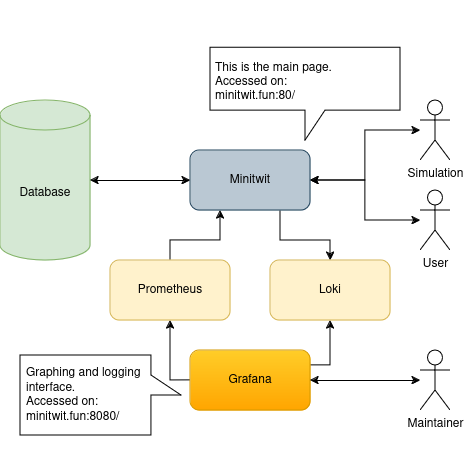
\includegraphics[scale=.7]{diagrams/context_diagram.png}
    \caption{Informal context diagram showing the connections between subsystems in the Minitwit system.}
    \label{fig:Informal context diagram}
\end{figure}

Figure \ref{fig:client_model_view} shows in more details how different clients interact with minitwit. The simulation has it's own endpoint. Users accessing the site through a web browser will get served a react frontend, which acts as an interface to communicate with the endpoints in the API. The endpoints do not directly speak to the database, but go through a repository structure which has different methods for accessing data in the database through the ORM.
\begin{figure}[H]
    \centering
    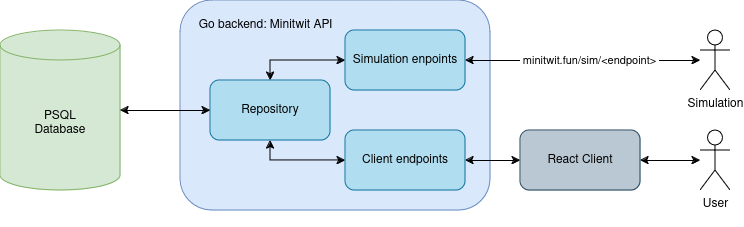
\includegraphics[width=\textwidth]{diagrams/Client_model_view.png}
    \caption{Client model view of the Minitwit application, showing how users interact with the React frontend, and the simulation interacts directly with the Go-lang backend.}
    \label{fig:client_model_view}
\end{figure}

Figure \ref{fig:register_sequence} shows a sequence diagram of how a successful registration of a new user is processed. A request is sent to the API. The API then checks with the database if the user already exists. The database returns that the user does not exist. The API then tells the database to create the new user. The API then increases it's metrics counter for new registrations. At last it returns to the client, in this case the simulator, that the user has been registered.
\begin{figure}[H]
    \centering
    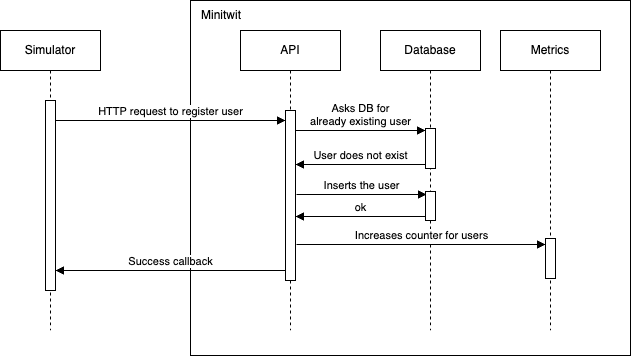
\includegraphics[width=\textwidth]{diagrams/register_sequence.png}
    \caption{Sequence diagram of the simulator registering a user.}
    \label{fig:register_sequence}
\end{figure}

